\documentclass[11pt, oneside]{article}   	% use "amsart" instead of "article" for AMSLaTeX format
\usepackage{geometry}                		% See geometry.pdf to learn the layout options. There are lots.
\geometry{letterpaper}                   		% ... or a4paper or a5paper or ... 
%\geometry{landscape}                		% Activate for for rotated page geometry
%\usepackage[parfill]{parskip}    		% Activate to begin paragraphs with an empty line rather than an indent
\usepackage{graphicx}				% Use pdf, png, jpg, or eps§ with pdflatex; use eps in DVI mode
								% TeX will automatically convert eps --> pdf in pdflatex		
\usepackage{amssymb}
\usepackage{amsmath}


\title{Reading List}
\author{Jon Eskreis-Winkler}
%\date{}							% Activate to display a given date or no date

\begin{document}
\maketitle
\input{/Users/jeffreywinkler/latex.tex}

\begin{center}\begin{tabular}{| l| l| l|} \hline
Fast Direct Methods for Gaussian Processes & Ambikasaran, Mackey, Greengard, Hogg, \textbf{O'Neil} & 2015 \\ \hline
\end{tabular}\end{center}
Background: Hierarchical off-diagonal low-rank (HODLR) matrices have a $k$-level hierarchy depicted by this:
\begin{center}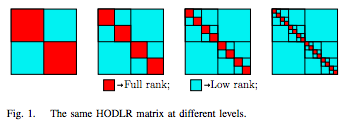
\includegraphics[scale=0.5]{HODLR.png} \end{center}
Motivation: Evaluating a Gaussian density amounts to dealing extensively with a matrix $C$ which is typically dense.
$$p(\theta|x,y) \propto p(y|\theta,x)p(\theta) \propto  \frac{1}{|\det(C(x))|^\frac{1}{2}} \exp \left(-\frac{1}{2} y^T C^{-1}(x)y \right)p(\theta)$$
The inversion and computation of determinant will take $O(n^3)$ operations. 
Result: When $C(x) = \sigma^2I+K(x)$ for a covariance matrix $K$ there may be a hierarchical factorization into a product of low-rank updates of the identity matrix. The resulting factorization permits inversion in $O(n\log^2 n)$ and determinant computation in $O(n\log n)$.
Key ideas:
\begin{itemize}
\item Even though the formulation of the factorization requires inversion of large sub-matrices matrices, there is a recursion within the large sub-matrices and in the end only small matrices get inverted.
\item Use good pictures to describe the structure of a factorization
\item Use Sylvester's Theorem to speed up determinant computations.
\item Use Sherman-Morrison-Woodbury Formula to invert small rank matrix updates to identity.
\end{itemize}
For additional reference see: 
\begin{verbatim}
/Users/jeffreywinkler/Google Drive/15fall/Kondor/Presentations/ONeil
\end{verbatim}

\begin{center}\begin{tabular}{| l| l| l|} \hline
Approximating GPs with $\mathcal{H}^2$ matrices & Borm Garcke & 2015 \\ \hline
\end{tabular}\end{center}
Background: Article deals with $\mathcal{H}$ and $\mathcal{H}^2$ matrices. 
\begin{itemize}
\item $\mathcal{H}$ matrices are used to provide low rank approximations. For example, given a dense matrix $M \in \mathbb{R}^{m\times n}$, storage will cost $O(mn)$. However, if we are able to approximate with a rank $k$ matrix $M\approx M^* = AB$ where $A \in \mathbb{R}^{m\times k}, \ B \in \mathbb{R}^{k\times n}$ then we can store an approximation $M^*$ in $O(mk+nk)= O(k(m+n))$.
\item $\mathcal{H}^2$ matrices replace the general low-rank structure of the blocks by a hierarchical representation closely related to the fast multipole method in order to reduce the storage complexity to $O(nk)$. Is this an improvement?
\end{itemize}
Motivation: Reconstructing $f: X\rightarrow Y$ using GP requires, in evaluation of the density $O(n^3)$ for direct methods and $O(n^2)$ for iterative methods. This makes large scale learning problems intractable. 
Result: Use Gaussian RBF kernel to make a matrix. Use $\mathcal{H}$ matrices as data-sparse approximations of the kernel matrix. This would reduce storage for $M \in \mathbb{R}^{N\times N}$ matrices to $O(Nm\log N)$ where $m$ is the rank of the local approximations (why the extra $\log N$?). $m$ will also determine accuracy. Also matrix multiplications will take $O(Nm\log N)$ and inverse (and determinant) is almost linear.

Key ideas:
\begin{itemize}
\item Kernel matrices may be full rank, but there is a natural and surprising factorization. For a matrix $K \in \mathbb{R}^{N\times N}$, $K_{i,j} = k(x_i,x_j)$. Using $m$ Lagrane polynomials $(\mathcal{L}_\nu)_{\nu=1}^m$ and $m$ interpolation points $(\xi_\nu)_{\nu=1}^m$, we approximate the kernel function as $\tilde k(x_i,x_j) = \sum_{\nu=1}^m L_\nu(x_i)k(\xi_\nu,x_j)$:
$$\tilde K = \begin{pmatrix} \mathcal{L}_1(x_1) & \cdots & \mathcal{L}_m(x_1)\\ \vdots & \ddots & \vdots\\ \mathcal{L}_1(x_N) & \cdots & \mathcal{L}_m(x_N)\\ \end{pmatrix}\begin{pmatrix} k(\xi_1,x_1) & \cdots & k(\xi_1, x_N) \\	 \vdots & \ddots & \vdots \\ 	 k(\xi_m,x_1) & \cdots & k(\xi_m,x_N) \\ \end{pmatrix}$$
When $k$ is a sufficiently smooth kernel, $m$ can be quite small.
\item This Lagrange-based factorization can be tough when $k$ is not globally smooth - only locally smooth. This would lead us to want to define sub-matrices to factorize in this way. The new task is to identify the sub-matrices to factor. The search is conducted by using binary space partitioning. The binary partitioning begins to be intractable for large dimensional data because there are so many border clusters. Barring this issue, finding the factorization has a complexity of $O(Nm\log N)$.
\item For $\mathcal{H}^2$ approximation, the factorization makes a stronger assumption, that both variables are interpolated. Mathematically, $\tilde k(x,y) = \sum_{\nu=1}^m \sum_{\mu=1}^m \mathcal{L}_\nu(x) k(\xi_\nu,\xi_\mu) \mathcal{L}_\mu(z)$. This introduces a "coupling matrix $S \in \mathbb{R}^{m\times m}$ and "cluster bases" $V,W \in \mathbb{R}^{N\times m}$ approximating $\tilde{K} = VSW^T =$
$$\begin{pmatrix} \mathcal{L}_1(x_1) & \cdots & \mathcal{L}_m(x_1)\\ \vdots & \ddots & \vdots\\ \mathcal{L}_1(x_N) & \cdots & \mathcal{L}_m(x_N)\\ \end{pmatrix}\begin{pmatrix} k(\xi_1,\xi_1) & \cdots & k(\xi_1, \xi_m) \\	 \vdots & \ddots & \vdots \\ 	 k(\xi_m,\xi_m) & \cdots & k(\xi_m,x_N) \\ \end{pmatrix} \begin{pmatrix} \mathcal{L}_1(x_1) & \cdots & \mathcal{L}_1(x_N)\\ \vdots & \ddots & \vdots\\ \mathcal{L}_m(x_1) & \cdots & \mathcal{L}_m(x_N)\\ \end{pmatrix}$$
The complexity of this approach to approximating $K$ is $O(Nm)$.
\item How to address the curse of dimensionality? "Coarsening"
\end{itemize}
Questions
\begin{itemize}
\item What is $m$ in the examples?
\item Seems to be polynomial?
\end{document}  
